\documentclass[11pt]{article}
\usepackage[margin=1in]{geometry}
\usepackage{booktabs}
\usepackage{tabularx}
\usepackage{array}
\usepackage{xcolor}
\usepackage{hyperref}
\usepackage{pgfplots}
\pgfplotsset{compat=1.18}
\usepackage{pgfplotstable}

% Right-aligned X column
\newcolumntype{Y}{>{\raggedleft\arraybackslash}X}

\hypersetup{colorlinks=true, linkcolor=blue, urlcolor=blue}

\begin{document}
\title{Startup Valuation Report — Hardcoded Version}
\author{Security-focused Bitcoin Subscription \& Hardware Model}
\date{\today}
\maketitle

% =========================================================
% EXECUTIVE OVERVIEW
% =========================================================
\section*{Executive Overview}
This document presents a hardcoded valuation model for a security service focused on Bitcoin users concerned with ``wrench attacks.'' Revenue comprises subscriptions and future proprietary hardware (which replaces subscriptions for adopters). Merchandise is treated only as CAC recoup, \emph{not} as revenue. Valuation uses ARR (subscriptions only) multiples.

% =========================================================
% CUSTOMER AVATAR (brief)
% =========================================================
\section{Customer Avatar (Brief)}
\begin{itemize}
  \item \textbf{Demographics:} 25--45, male-skewed, urban/suburban in higher-adoption markets (U.S., Germany, LATAM, parts of Asia).
  \item \textbf{Psychographics:} Sovereignty/privacy-first; distrusts custodians; pays for risk reduction.
  \item \textbf{Behavior:} Active on X/Reddit/Telegram/Podcasts; buys VPNs/hardware wallets.
  \item \textbf{Primary pain:} Physical coercion risk (``\$5 wrench attack'').
\end{itemize}

% =========================================================
% CORE INPUT PARAMETERS (HARDCODED)
% =========================================================
\section{Core Input Parameters}

\subsection*{Subscription Tiers \& Distribution}
\begin{tabularx}{\linewidth}{l Y Y Y}
\toprule
Tier & Price (/mo) & Mix (\%) & Monthly revenue / user \\\midrule
Basic   & 2.60  & 90 & 2.34 \\
Medium  & 30.00 & 9  & 2.70 \\
Golden  & 220.00& 1  & 2.20 \\\midrule
\textbf{Totals / Avg} &  & \textbf{100} & \textbf{7.24} \\
\bottomrule
\end{tabularx}

\subsection*{Derived Metrics (Subscriptions Only)}
\begin{tabularx}{\linewidth}{l Y}
\toprule
Metric & Value (USD) \\\midrule
Monthly ARPU & 7.24 \\
Annual ARPU  & 86.88 \\
\bottomrule
\end{tabularx}

\subsection*{Hardware Pricing, Margins \& Mix}
\begin{tabularx}{\linewidth}{l Y Y Y}
\toprule
Device & Retail (USD) & Margin (\%) & Mix (\%) \\\midrule
Entry        & 500  & 40 & 60 \\
Professional & 1000 & 45 & 30 \\
Premium      & 2000 & 50 & 10 \\\midrule
\textbf{Weighted Avg GP / device} & \multicolumn{3}{r}{\textbf{355}} \\
\bottomrule
\end{tabularx}

\subsection*{Capital \& CAC (Merch recoups CAC; merch not revenue)}
\begin{tabularx}{\linewidth}{l Y Y Y Y}
\toprule
Parameter & Ticket (USD) & Dev (USD) & Marketing (USD) & Target Valuation (USD) \\\midrule
Inputs & 150{,}000 & 50{,}000 & 100{,}000 & 5{,}000{,}000 \\
Stake Offered (\%) & \multicolumn{4}{r}{3} \\
\bottomrule
\end{tabularx}

\begin{tabularx}{\linewidth}{l Y Y Y Y}
\toprule
CAC Param & Gross CAC (USD) & Merch Recoup (\%) & \textbf{Effective CAC} (USD) & Users from \$100k \\\midrule
Values & 20 & 50 & \textbf{10} & \textbf{10{,}000} \\
\bottomrule
\end{tabularx}

\subsection*{Adoption, Growth, and Valuation Multiples}
\begin{tabularx}{\linewidth}{l Y}
\toprule
Parameter & Value \\\midrule
Hardware adoption per year (starting Year 2; replaces subs) & 5\% \\
Valuation Multiples (Conservative / Moderate / Optimistic) & 5x / 7x / 10x \\
\bottomrule
\end{tabularx}

% =========================================================
% YEAR 1 SNAPSHOT
% =========================================================
\section{Year 1 Snapshot (Subscriptions only; hardware not yet selling)}
\begin{tabularx}{\linewidth}{l Y Y Y}
\toprule
Scenario & Users (Y1) & ARR Subs (Y1, USD) & Valuation (Multiple) \\\midrule
Conservative & 2{,}000  & 173{,}760 & 868{,}800 (5x) \\
Moderate     & 10{,}000 & 868{,}800 & 6{,}081{,}600 (7x) \\
Optimistic   & 50{,}000 & 4{,}344{,}000 & 43{,}440{,}000 (10x) \\
\bottomrule
\end{tabularx}

% =========================================================
% THREE-YEAR PROJECTION (BASELINE)
% =========================================================
\section{Three-Year Projection (Baseline)}
Assumptions: linear total-user growth per year; hardware sales start in Year 2 and \textbf{replace} subs for adopters (5\% of total users per year).

\subsection*{Total Users and Subscribing Users}
\begin{tabularx}{\linewidth}{l Y Y Y Y Y Y}
\toprule
 & \multicolumn{3}{c}{Total Users} & \multicolumn{3}{c}{Subscribing Users} \\
Scenario & Y1 & Y2 & Y3 & Y1 & Y2 & Y3 \\\midrule
Conservative (+1{,}500/yr) & 2{,}000 & 3{,}500 & 5{,}000 & 2{,}000 & 3{,}325 & 4{,}500 \\
Moderate (+10{,}000/yr)    & 10{,}000 & 20{,}000 & 30{,}000 & 10{,}000 & 19{,}000 & 27{,}000 \\
Optimistic (+25{,}000/yr)  & 50{,}000 & 75{,}000 & 100{,}000 & 50{,}000 & 71{,}250 & 90{,}000 \\
\bottomrule
\end{tabularx}

\subsection*{ARR (Subscriptions Only) and Hardware Gross Profit (One-off)}
\begin{tabularx}{\linewidth}{l Y Y Y Y Y Y}
\toprule
 & \multicolumn{3}{c}{ARR Subs (USD)} & \multicolumn{3}{c}{Hardware GP (USD)} \\
Scenario & Y1 & Y2 & Y3 & Y1 & Y2 & Y3 \\\midrule
Conservative & 173{,}760 & 288{,}876 & 390{,}960 & 0 & 62{,}125 & 88{,}750 \\
Moderate     & 868{,}800 & 1{,}650{,}720 & 2{,}345{,}760 & 0 & 355{,}000 & 532{,}500 \\
Optimistic   & 4{,}344{,}000 & 6{,}190{,}200 & 7{,}819{,}200 & 0 & 1{,}331{,}250 & 1{,}775{,}000 \\
\bottomrule
\end{tabularx}

\subsection*{Valuation (Multiple $\times$ ARR, Subscriptions Only)}
\begin{tabularx}{\linewidth}{l Y Y Y}
\toprule
Scenario & Valuation Y1 (USD) & Valuation Y2 (USD) & Valuation Y3 (USD) \\\midrule
Conservative (5x) & 868{,}800 & 1{,}444{,}380 & 1{,}954{,}800 \\
Moderate (7x)     & 6{,}081{,}600 & 11{,}555{,}040 & 16{,}420{,}320 \\
Optimistic (10x)  & 43{,}440{,}000 & 61{,}902{,}000 & 78{,}192{,}000 \\
\bottomrule
\end{tabularx}

% =========================================================
% REPUTATIONAL BOOST SCENARIO
% =========================================================
\section{Reputational Boost Scenario}
Assumptions changed vs.\ baseline:
\begin{itemize}
  \item Annual user additions \textbf{double}: +3{,}000 / +20{,}000 / +50{,}000 (Cons / Mod / Opt).
  \item Hardware adoption still 5\%/yr from Year 2 and still replaces subscriptions.
  \item ARPU unchanged (86.88 USD per subscriber per year) for comparability.
\end{itemize}

\subsection*{Total Users and Subscribing Users (Boost)}
\begin{tabularx}{\linewidth}{l Y Y Y Y Y Y}
\toprule
 & \multicolumn{3}{c}{Total Users} & \multicolumn{3}{c}{Subscribing Users} \\
Scenario & Y1 & Y2 & Y3 & Y1 & Y2 & Y3 \\\midrule
Conservative (+3{,}000/yr) & 2{,}000 & 5{,}000 & 8{,}000 & 2{,}000 & 4{,}750 & 7{,}200 \\
Moderate (+20{,}000/yr)    & 10{,}000 & 30{,}000 & 50{,}000 & 10{,}000 & 28{,}500 & 45{,}000 \\
Optimistic (+50{,}000/yr)  & 50{,}000 & 100{,}000 & 150{,}000 & 50{,}000 & 95{,}000 & 135{,}000 \\
\bottomrule
\end{tabularx}

\subsection*{ARR (Subscriptions Only, Boost)}
\begin{tabularx}{\linewidth}{l Y Y Y}
\toprule
Scenario & ARR Y1 (USD) & ARR Y2 (USD) & ARR Y3 (USD) \\\midrule
Conservative & 173{,}760 & 412{,}680 & 625{,}536 \\
Moderate     & 868{,}800 & 2{,}476{,}080 & 3{,}909{,}600 \\
Optimistic   & 4{,}344{,}000 & 8{,}253{,}600 & 11{,}728{,}800 \\
\bottomrule
\end{tabularx}

\subsection*{Valuation Impact (Boost)}
\begin{tabularx}{\linewidth}{l Y Y Y}
\toprule
Scenario & Valuation Y1 (USD) & Valuation Y2 (USD) & Valuation Y3 (USD) \\\midrule
Conservative (5x) & 868{,}800 & 2{,}063{,}400 & 3{,}127{,}680 \\
Moderate (7x)     & 6{,}081{,}600 & 17{,}332{,}560 & 27{,}367{,}200 \\
Optimistic (10x)  & 43{,}440{,}000 & 82{,}536{,}000 & 117{,}288{,}000 \\
\bottomrule
\end{tabularx}

% =========================================================
% SANITY CHECK: TICKET, CAC, AND TARGET
% =========================================================
\section{Sanity Check: Ticket, CAC, and Target}
\begin{itemize}
  \item Ticket \$150k for 3\% \Rightarrow \$5.0M post-money target.
  \item \$50k dev; \$100k marketing.
  \item Gross CAC \$20; 50\% merch recoup \Rightarrow effective CAC \$10.
  \item Users acquired from \$100k at \$10 each \Rightarrow \textbf{10{,}000} users.
  \item ARR impact before replacement: 10{,}000 $\times$ 86.88 = \$868{,}800. At 7$\times$ multiple = \$6.08M. With modest replacement into hardware (still one-off GP, not ARR), practical mid-year valuation \emph{near} \$5M in the moderate case is credible.
\end{itemize}

% =========================================================
% GRAPHS (HARDCODED)
% =========================================================
\section{Graphs (Hardcoded)}

\begin{figure}[h!]
\centering
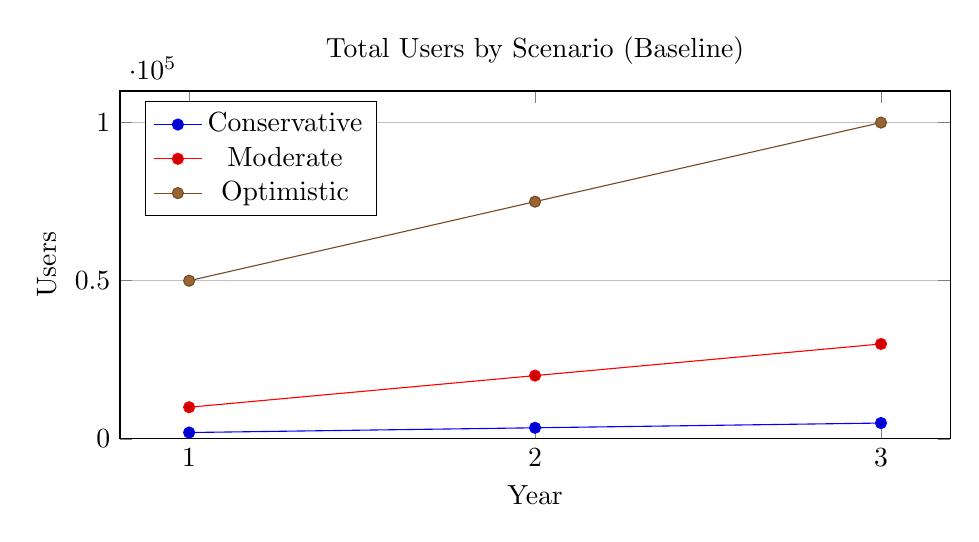
\begin{tikzpicture}
\begin{axis}[
  width=\linewidth,
  height=6cm,
  xlabel={Year},
  ylabel={Users},
  xtick={1,2,3},
  ymin=0,
  legend pos=north west,
  ymajorgrids,
  title={Total Users by Scenario (Baseline)}
]
\addplot+[mark=*] coordinates {(1,2000) (2,3500) (3,5000)};
\addlegendentry{Conservative}
\addplot+[mark=*] coordinates {(1,10000) (2,20000) (3,30000)};
\addlegendentry{Moderate}
\addplot+[mark=*] coordinates {(1,50000) (2,75000) (3,100000)};
\addlegendentry{Optimistic}
\end{axis}
\end{tikzpicture}
\caption{Total users over 3 years (baseline).}
\end{figure}

\begin{figure}[h!]
\centering
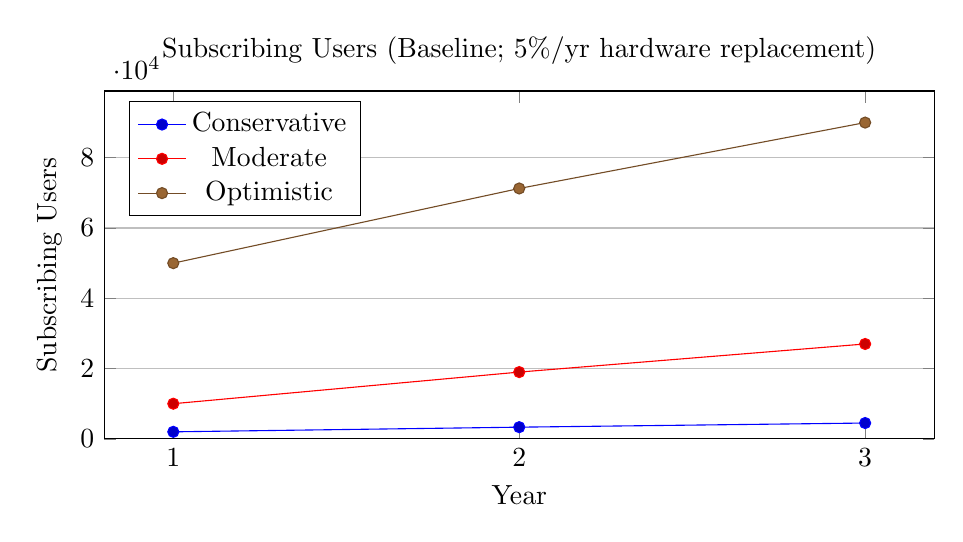
\begin{tikzpicture}
\begin{axis}[
  width=\linewidth,
  height=6cm,
  xlabel={Year},
  ylabel={Subscribing Users},
  xtick={1,2,3},
  ymin=0,
  legend pos=north west,
  ymajorgrids,
  title={Subscribing Users (Baseline; 5\%/yr hardware replacement)}
]
\addplot+[mark=*] coordinates {(1,2000) (2,3325) (3,4500)};
\addlegendentry{Conservative}
\addplot+[mark=*] coordinates {(1,10000) (2,19000) (3,27000)};
\addlegendentry{Moderate}
\addplot+[mark=*] coordinates {(1,50000) (2,71250) (3,90000)};
\addlegendentry{Optimistic}
\end{axis}
\end{tikzpicture}
\caption{Subscribing users decline relative to total as hardware replaces subs.}
\end{figure}

\begin{figure}[h!]
\centering
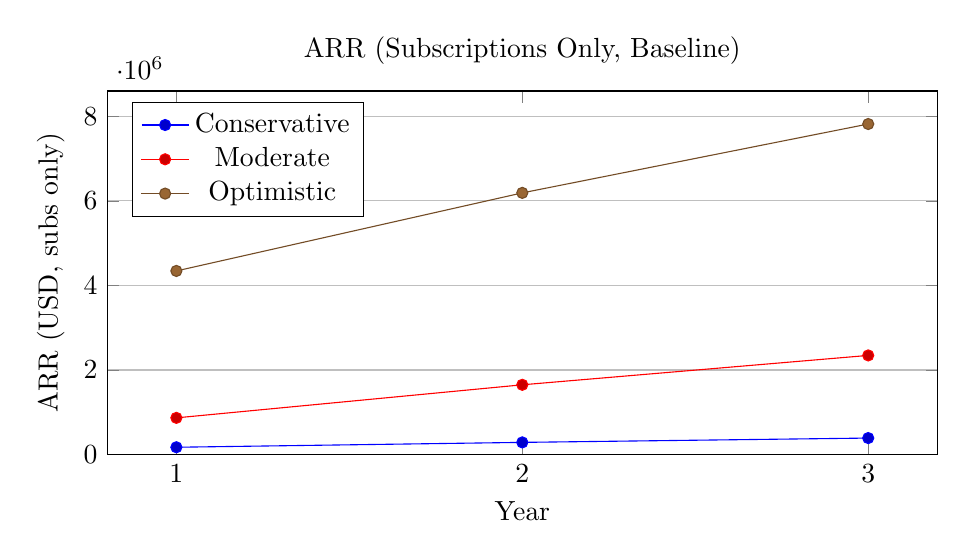
\begin{tikzpicture}
\begin{axis}[
  width=\linewidth,
  height=6.2cm,
  xlabel={Year},
  ylabel={ARR (USD, subs only)},
  xtick={1,2,3},
  ymin=0,
  ymajorgrids,
  legend pos=north west,
  title={ARR (Subscriptions Only, Baseline)}
]
\addplot+[mark=*] coordinates {(1,173760) (2,288876) (3,390960)};
\addlegendentry{Conservative}
\addplot+[mark=*] coordinates {(1,868800) (2,1650720) (3,2345760)};
\addlegendentry{Moderate}
\addplot+[mark=*] coordinates {(1,4344000) (2,6190200) (3,7819200)};
\addlegendentry{Optimistic}
\end{axis}
\end{tikzpicture}
\caption{ARR excludes hardware (one-off) by design; valuation uses ARR multiples.}
\end{figure}

\begin{figure}[h!]
\centering
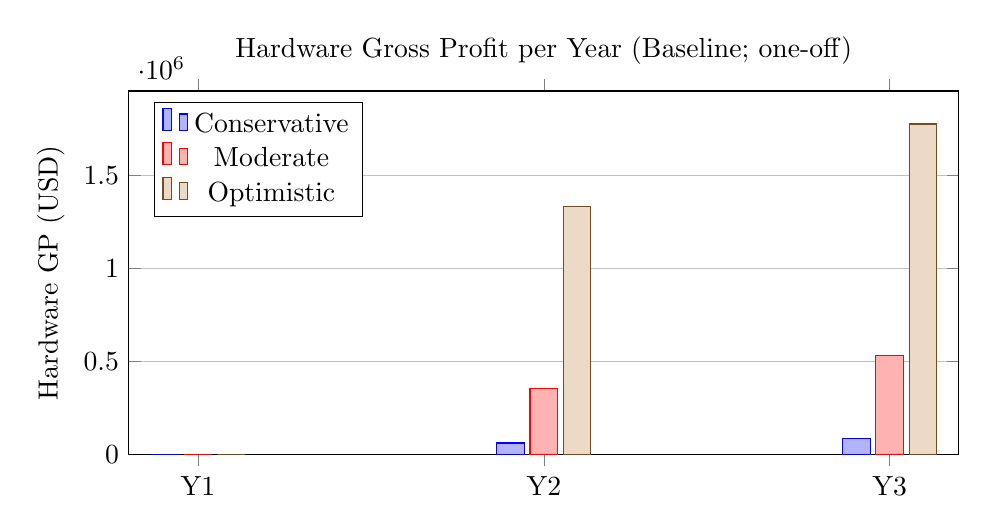
\begin{tikzpicture}
\begin{axis}[
  ybar,
  width=\linewidth,
  height=6.2cm,
  bar width=10pt,
  symbolic x coords={Y1,Y2,Y3},
  xtick=data,
  ylabel={Hardware GP (USD)},
  ymin=0,
  ymajorgrids,
  legend pos=north west,
  title={Hardware Gross Profit per Year (Baseline; one-off)}
]
\addplot coordinates {(Y1,0) (Y2,62125) (Y3,88750)};
\addlegendentry{Conservative}
\addplot coordinates {(Y1,0) (Y2,355000) (Y3,532500)};
\addlegendentry{Moderate}
\addplot coordinates {(Y1,0) (Y2,1331250) (Y3,1775000)};
\addlegendentry{Optimistic}
\end{axis}
\end{tikzpicture}
\caption{Hardware GP shown separately (not part of ARR).}
\end{figure}

\begin{figure}[h!]
\centering
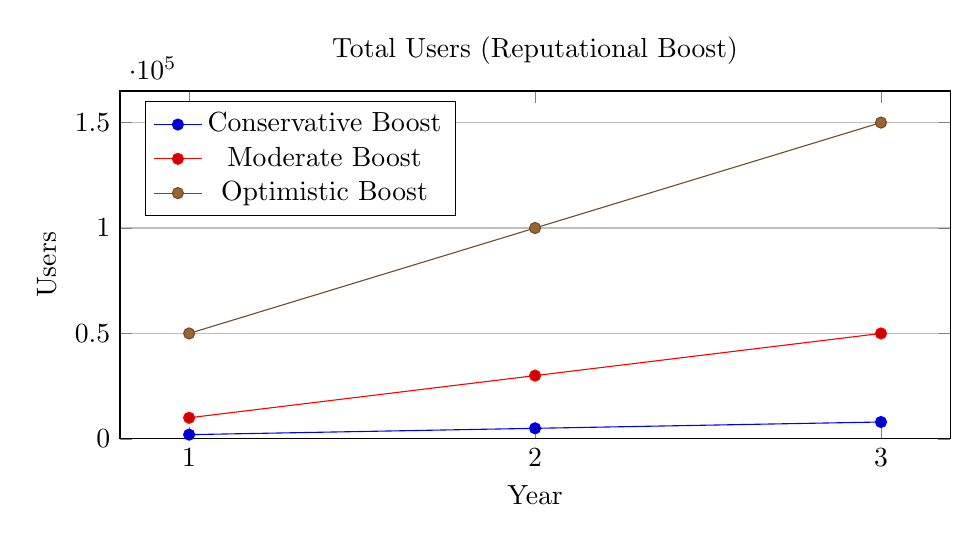
\begin{tikzpicture}
\begin{axis}[
  width=\linewidth,
  height=6cm,
  xlabel={Year},
  ylabel={Users},
  xtick={1,2,3},
  ymin=0,
  legend pos=north west,
  ymajorgrids,
  title={Total Users (Reputational Boost)}
]
\addplot+[mark=*] coordinates {(1,2000) (2,5000) (3,8000)};
\addlegendentry{Conservative Boost}
\addplot+[mark=*] coordinates {(1,10000) (2,30000) (3,50000)};
\addlegendentry{Moderate Boost}
\addplot+[mark=*] coordinates {(1,50000) (2,100000) (3,150000)};
\addlegendentry{Optimistic Boost}
\end{axis}
\end{tikzpicture}
\caption{Reputational investor pulls adoption forward (higher inflows earlier).}
\end{figure}

\begin{figure}[h!]
\centering
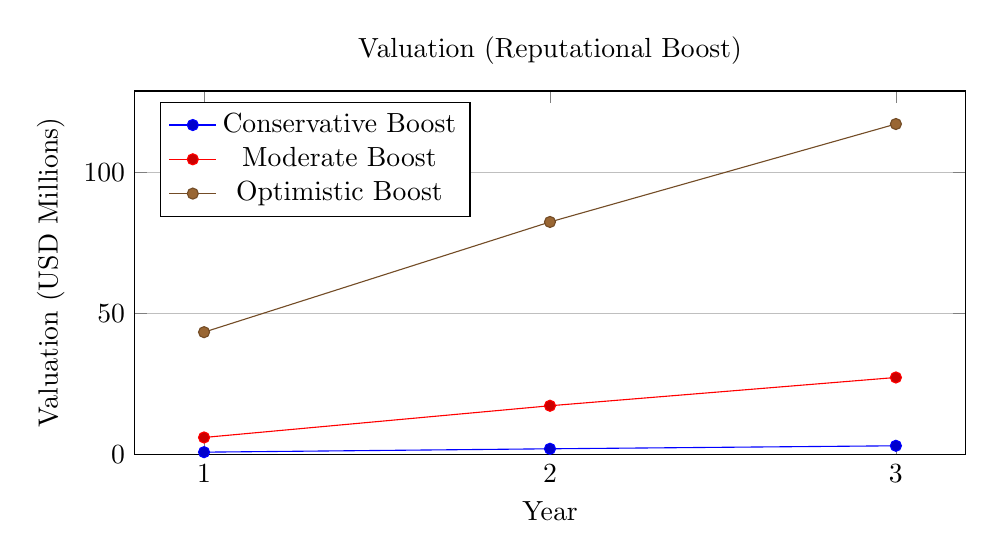
\begin{tikzpicture}
\begin{axis}[
  width=\linewidth,
  height=6.2cm,
  xlabel={Year},
  ylabel={Valuation (USD Millions)},
  xtick={1,2,3},
  ymin=0,
  ymajorgrids,
  legend pos=north west,
  title={Valuation (Reputational Boost)}
]
\addplot+[mark=*] coordinates {(1,0.8688) (2,2.0634) (3,3.12768)};
\addlegendentry{Conservative Boost}
\addplot+[mark=*] coordinates {(1,6.0816) (2,17.33256) (3,27.3672)};
\addlegendentry{Moderate Boost}
\addplot+[mark=*] coordinates {(1,43.44) (2,82.536) (3,117.288)};
\addlegendentry{Optimistic Boost}
\end{axis}
\end{tikzpicture}
\caption{Boost raises valuations earlier using the same ARR multiples.}
\end{figure}

\end{document}
